Para este caso, a simulação numérica é realizada para uma artéria coronária
real com aterosclerose cuja geometria foi obtida através de um processamento de imagem
como sugerido por Wang et al. (2017) \cite{wang2017}. Essa geometria é particular para
cada paciente devido as condições de saúde do mesmo. 
Assim como nos casos anteriores, foi considerado uma obstrução
de 40\% do canal devido a aterosclerose e o domínio foi
discretizado com 7632 nós e 14665 elementos triangulares lineares. \par
A \ref{velocity evolution real} apresenta o perfil
de velocidade transiente ao longo da coordenada $y$ no
meio do canal ($x=5R$). 
O valor adimensional máximo do campo de velocidade chega
a $u=2.25$. Dessa forma, a geometria curvada representa
uma boa aproximação como observado na \ref{velocity evolution curved}.



\begin{figure}[H]
     \centering
     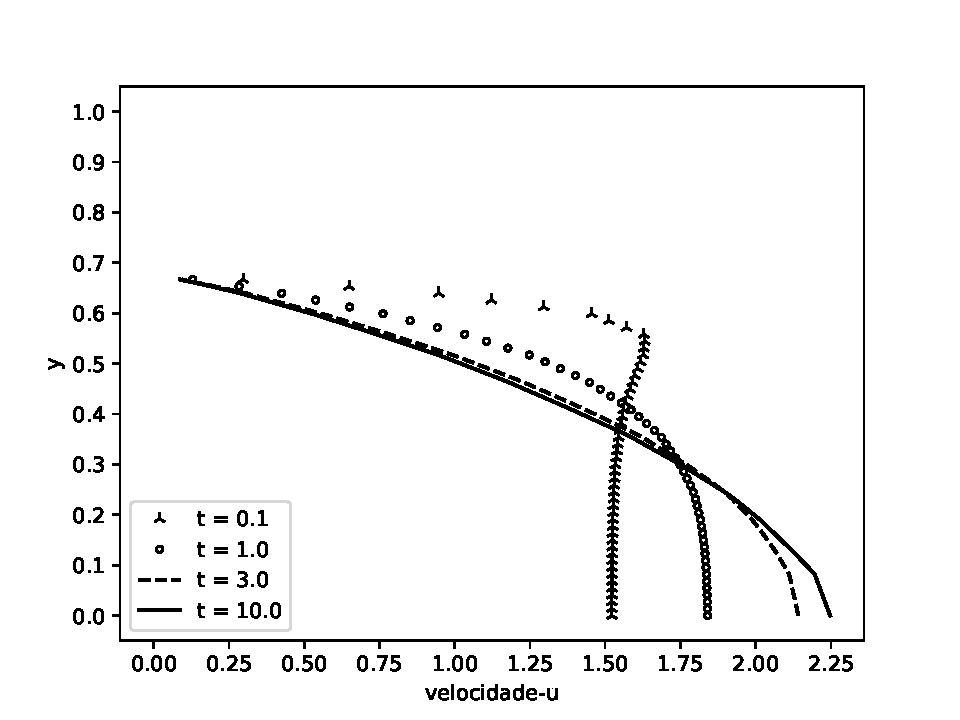
\includegraphics[scale=1]{./02_chaps/cap_solution/figure/vel_Real_evol.pdf}\\
     \caption{Evolução no tempo do perfil da velocidade para o Canal Real.}
     \label{velocity evolution real}
\end{figure}

\newpage
A \ref{velocity field real} apresenta a evolução no tempo e no espaço
do campo de velocidade para a metade do domínio já que os resultados são simétricos
na direção $y$. O campo de velocidade é representado com os valores adimensionais
onde a cor vermelha se refere ao valor $u=2.25$ e a cor azul $u=0$.

\vspace{2cm} 
\begin{figure}[H]
     \begin{minipage}{.50\linewidth}
      \centering
      
\includegraphics[scale=0.12]{./02_chaps/cap_solution/figure/vel_Real200.png}\\
      t = 0.1
     \end{minipage}%
     \begin{minipage}{.50\linewidth}
      \centering
      
\includegraphics[scale=0.12]{./02_chaps/cap_solution/figure/vel_Real1000.png}\\
      t = 0.5
     \end{minipage}
     \begin{minipage}{.50\linewidth}
     \medskip
      \centering
      
\includegraphics[scale=0.12]{./02_chaps/cap_solution/figure/vel_Real2000.png}\\
      t = 1.0
     \end{minipage}%
     \begin{minipage}{.50\linewidth}
     \medskip
      \centering
      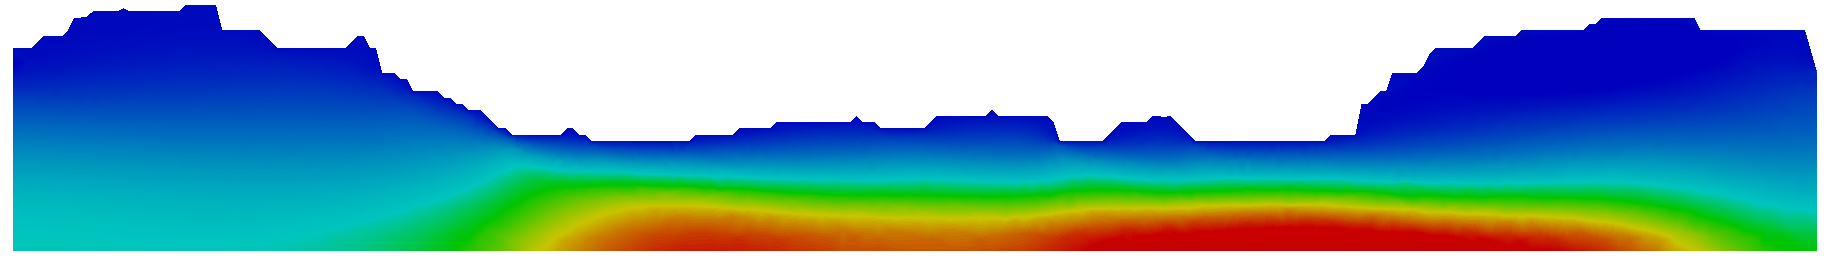
\includegraphics[scale=0.12]{./02_chaps/cap_solution/figure/vel_Real6000.png}\\
      t = 3.0
     \end{minipage}
     \begin{minipage}{.50\linewidth}
      \centering
      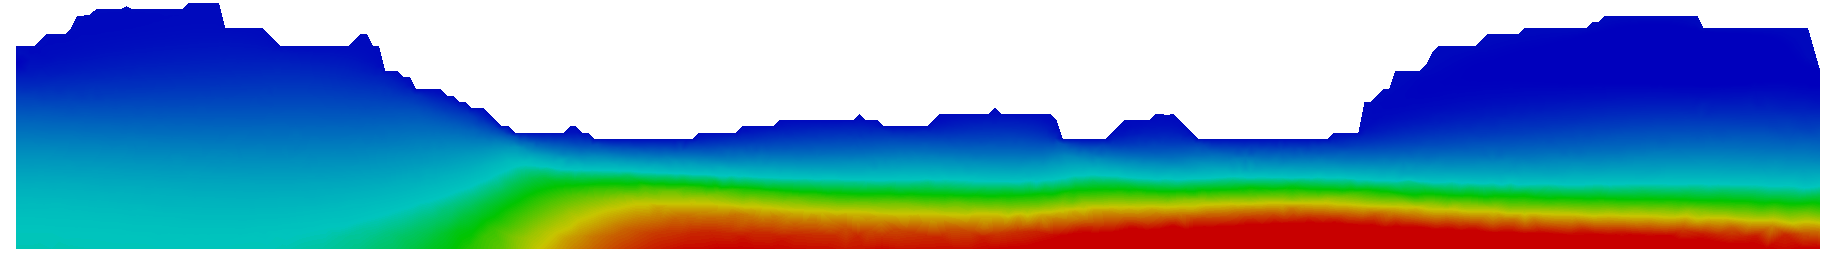
\includegraphics[scale=0.12]{./02_chaps/cap_solution/figure/vel_Real8000.png}\\
      t = 4.0
     \end{minipage}%
     \begin{minipage}{.50\linewidth}
      \centering
      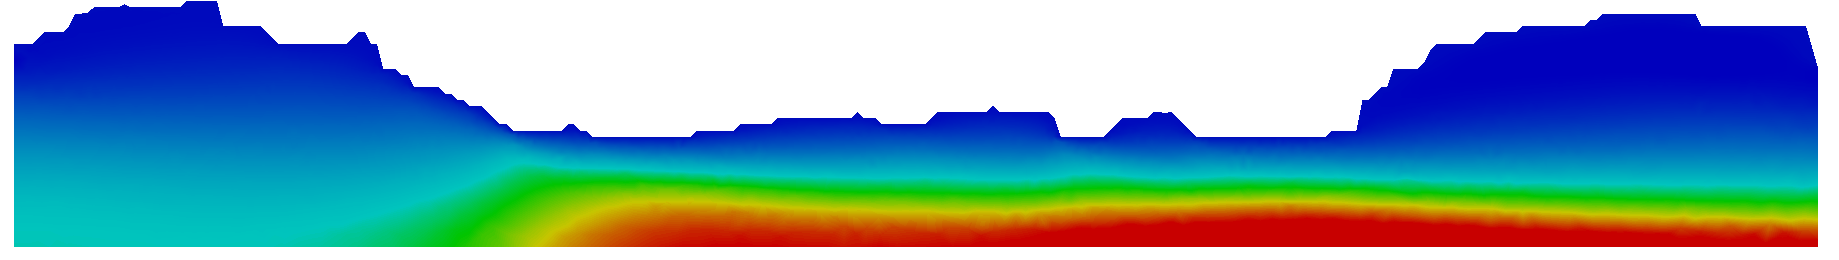
\includegraphics[scale=0.12]{./02_chaps/cap_solution/figure/vel_Real10000.png}\\
      t = 5.0
     \end{minipage}
     \begin{minipage}{.50\linewidth}
     \medskip
      \centering
      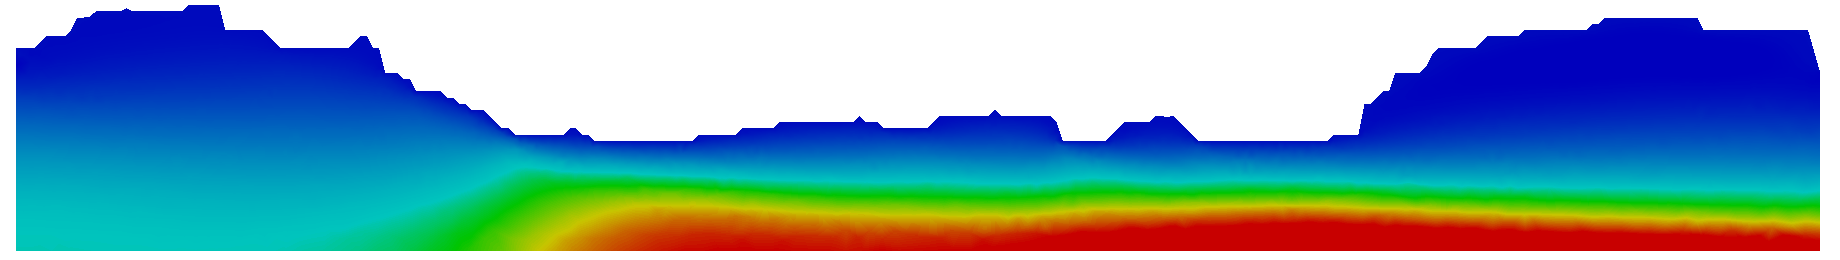
\includegraphics[scale=0.12]{./02_chaps/cap_solution/figure/vel_Real14000.png}\\
      t = 7.0
     \end{minipage}%
     \begin{minipage}{.50\linewidth}
     \medskip
      \centering
      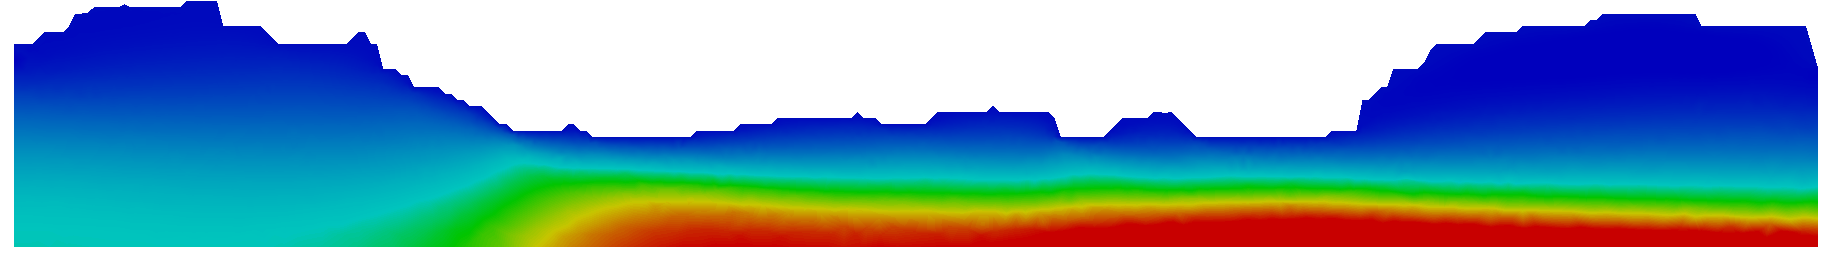
\includegraphics[scale=0.12]{./02_chaps/cap_solution/figure/vel_Real20000.png}\\
      t = 10.0
     \end{minipage}
     \medskip
     \caption{Evolução no tempo e no espaço do campo de velocidade para o Canal Real.}
     \label{velocity field real}
\end{figure}

\newpage
